\section{Implementasjon}
\subsection{Beskrivelse av kode}
Koden starter selvfølgelig med å importere de nødvendige pakkene som trengs for å bruke spesielle funksjoner til å blant annet opprette en socket og kommunisere med serveren. Denne klienten bruker disse 7 pakkene:
\begin{lstlisting}
	import java.io.InputStreamReader;
	import java.io.BufferedReader;
	import java.io.IOException;
	import java.io.PrintStream;
	import java.net.Socket;
	import java.net.InetAddress;
	import java.util.Scanner;
\end{lstlisting}

Det finnes en alternativ måte å importere pakker på, hvor man skriver \textbf{import java.io.*} for å importere alle klassene som ligger inne i pakken. Fordelen med denne metoden er at man sparer noen linjer og man slipper å huske de forskjellige pakkenavnene. Ulempen derimot er at koden bruker mer tid under kompilering og bruker generelt mer plass. Derfor er det med andre ord lurest å kun importere de pakkene man trenger.\\

Alle funksjonene i TCP klienten er lagt inn i en klasse kalt TCPClient, hvor alle private variabler ligger øverst i klassen. Den første funksjonen som kjøres er da selvfølgelig \textbf{void main()}:
\begin{lstlisting}
	public class TCPClient{
		private Socket sock;
		private String ip;
		private int port;
		private char bufferIn[] = new char[512];
		private char bufferOut[] = new char[10];
		
		public static void main(String args[]) throws Exception{
			try{
				TCPClient client = new TCPClient();
				client.askUser();
				client.createSocket();
				client.sendData();
				client.readData();
			}
		}
	}
\end{lstlisting}

Dersom noen av disse funksjonene feiler og ikke klarer å kjøre så vil funksjonen kaste en exception, altså en feilmelding som tas imot nederst i koden:
\begin{lstlisting}
	catch(Exception e){
		System.out.println("ERROR: Something went wrong!");
	}
\end{lstlisting}

Det er totalt fem funksjoner i klienten, og før disse kjøres så opprettes det en instans av klassen, for å allokere nok plass i minnet til det objektet som nettopp ble opprettet. Vi kan deretter kjøre funksjonene som ligger i objektet ved å skrive:
\begin{lstlisting}
	TCPClient client = new TCPClient();
	client.askUser();
	client.createSocket();
	client.sendData();
	client.readData();
\end{lstlisting}

Den første funksjonen som kjøres er \textbf{askUser()}. Denne funksjonen spør brukeren om å skrive inn serverens IP addresse og port nummer. Dersom IP og port er gyldig så får de private variablene verdien av disse. Ved feil vil det kastes en exception, altså en feilmelding som vises før programmet avsluttes.
\begin{lstlisting}
	private void askUser() throws Exception{
		System.out.print("Enter the server IP address: ");
		Scanner input = new Scanner(System.in);
		String tmpIP = input.nextLine();
		if(tmpIP == "lekeplass") ip = "158.36.70.56"; else ip = tmpIP;

		System.out.print("Enter the server port: ");
		int tmpPort = input.nextInt();
		if(tmpPort <= 0 || tmpPort > 99999) System.out.println("ERROR: Invalid port!");
		else port = tmpPort;
	}
\end{lstlisting}

Etter at IP adressen og port er satt så kjøres neste funksjon, altså \textbf{createSocket()}. Denne funksjonen oppretter en socket mellom klient og server ved bruk av gitt IP adresse og port. Dersom klienten får kontakt med serveren, vil den forsøke å koble seg til. Dette gjøres ved hjelp av klassen \textbf{Socket} som ligger inne i pakken \textbf{java.net.Socket}, som vi inkluderte i begynnelsen av programmet.
\begin{lstlisting}
	private void createSocket() throws Exception{
		InetAddress address = InetAddress.getByName(ip);
		sock = new Socket(address, port);
	}
\end{lstlisting}

Nå er det opprettet en socket mellom klient og server, og klienten kan nå kommunisere med serveren. Serveren er satt opp med en spesifikk protokoll som kun godtar en liste med 10 bytes. Slik det er beskrevet i oppgaven så trenger man en melding ID, størrelse på meldingen, størrelsen på studentnummer og i tillegg sende studentnummer til serveren, og deretter vil serveren sjekke om klienten ber om riktig kommando, eventuelt om det er oppgitt feil studentnummer.\\

I \textbf{sendData()} funksjonen blir disse verdiene satt inn i et array bestående av characters. Melding ID er en \textit{char}, altså 1 byte, det samme gjelder størrelsen av studentnummer, mens størrelsen av meldingen er en \textit{short}, altså 2 bytes. Sammen med studentnummer som består av 6 characters, så har vi en liste med tilsammen 10 bytes. Denne lista sendes videre til serveren ved hjelp av klassen PrintStream, som tar dataen som ligger inne i arrayet og overfører dette videre til serveren.
\begin{lstlisting}
	private void sendData() throws Exception{
		char msg_id = 0x01;
		short msg_size = 7;
		char studnr_size = 6;

		bufferOut[0] = msg_id; // Message ID
		bufferOut[1] = 0; // Size of stream (Big endian)
		bufferOut[2] = (char)msg_size; // Size of stream (Big endian)
		bufferOut[3] = studnr_size; // Size of studentnr
		
		System.out.print("Enter your student number: ");
		Scanner input = new Scanner(System.in);
		String studnr = input.next();
		for(int i = 0; i < studnr.length(); i++) bufferOut[i+4] = studnr.charAt(i);
		
		PrintStream ps = new PrintStream(sock.getOutputStream());
		ps.println(bufferOut);
	}
\end{lstlisting}

Siste funksjon er å motta data fra serveren, altså motta en tilbakemelding på om vi har brukt riktig kommando, eller om vi har oppgitt riktig studentnummer. Dersom alle kravene er oppfylt og vi har sendt inn riktig data, vil serveren returnere oppgaveteksten til obligatorisk innlevering 2. Denne teksten leses i form av characters, som oppbevares i et buffer som har nok plass å oppbevare 512 characters. Når oppgaveteksten er mottatt, printes den ut og deretter avsluttes programmet.
\begin{lstlisting}
	private void readData() throws Exception{
		InputStreamReader isr = new InputStreamReader(sock.getInputStream());
		BufferedReader br = new BufferedReader(isr);
		br.read(bufferIn, 0, bufferIn.length);
		System.out.print(bufferIn);
	}
\end{lstlisting}

\subsection{Demonstrasjon}
I figuren under har vi koblet til serveren med riktig IP adresse og port, og deretter oppgitt riktig studentnummer. Serveren vil da altså returnere oppgaveteksten til oblig 2.\\\\
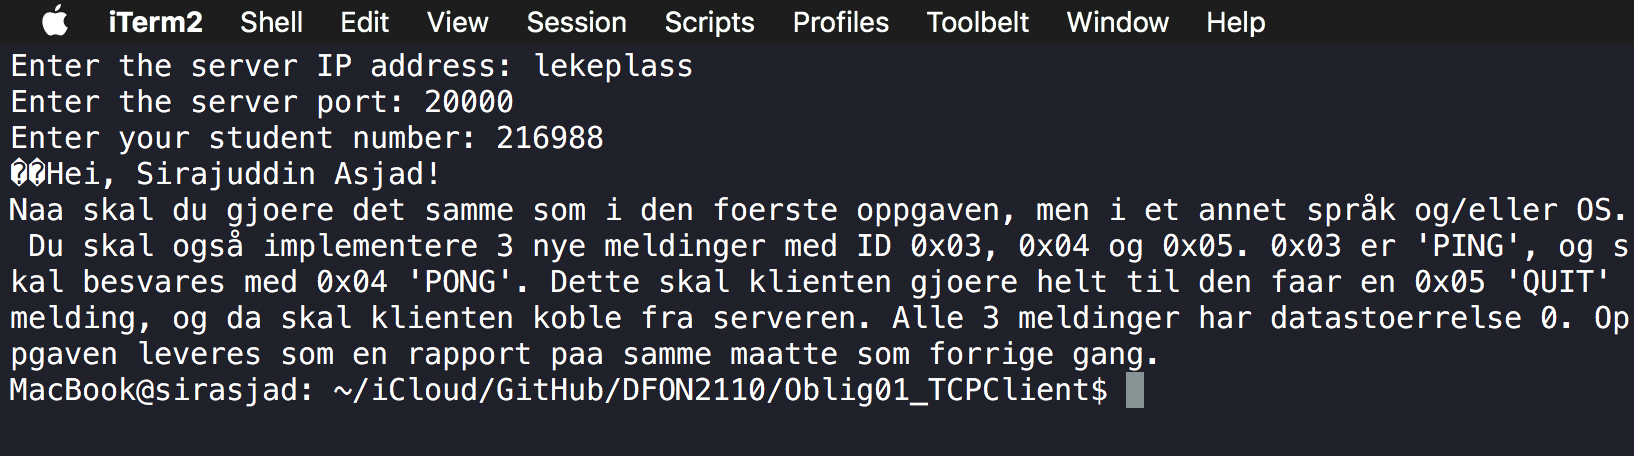
\includegraphics[width=\textwidth]{demo}
